\documentclass[UTF8,a4paper,12pt]{ctexart}

\usepackage{geometry}
\usepackage{graphicx}
\usepackage{booktabs}
\usepackage{longtable}
\usepackage{array}
\usepackage{float}
\usepackage{amsmath}
\usepackage{xcolor}
\usepackage{listings}
\usepackage{hyperref}
\usepackage{caption}
\usepackage{setspace}
\usepackage{xurl}
\usepackage{fontspec}

\setmainfont{Times New Roman}
\setsansfont{Times New Roman}
\setCJKmainfont[AutoFakeBold=2.5,AutoFakeSlant=0.2]{SimSun}
\setCJKsansfont[AutoFakeBold=2.5,AutoFakeSlant=0.2]{SimSun}
\setCJKmonofont{SimSun}

\geometry{left=2.6cm,right=2.6cm,top=2.5cm,bottom=2.5cm}
\onehalfspacing
\emergencystretch=2em
\urlstyle{tt}
\hypersetup{colorlinks=true,linkcolor=blue,urlcolor=blue}
\setlength{\parindent}{2em}
\setlength{\parskip}{0.25em}
\captionsetup{font=small,labelfont=normalfont,textfont=normalfont}
\setlength{\intextsep}{8pt plus 2pt minus 2pt}
\setlength{\textfloatsep}{10pt plus 2pt minus 2pt}
\setlength{\floatsep}{8pt plus 2pt minus 2pt}

\lstset{
  basicstyle=\ttfamily\small,
  breaklines=true,
  frame=single,
  columns=fullflexible,
  keywordstyle=\color{blue},
  commentstyle=\color{gray},
  stringstyle=\color{teal},
  showstringspaces=false
}

\begin{document}

\begin{titlepage}
\centering
\vspace*{2.2cm}
{\zihao{1}\bfseries 传感器与检测技术实验报告\par}
\vspace{1.2cm}
{\zihao{2}\bfseries 实验六：BMP280 气压测高与高度融合\par}
\vspace{2.2cm}
\begin{tabular}{rl}
课程名称：& 传感器与检测技术\\[0.6cm]
实验对象：& ESP32 + BMP280 气压传感器 + GPS 模块\\[0.6cm]
开发方式：& MicroPython + Python 后处理 + LaTeX 排版\\[0.6cm]
姓名：& 罗丹\\[0.6cm]
学号：& 2251801014\\[0.6cm]
GitHub：& \url{https://github.com/gf-be/ESP32_course}\\[0.6cm]
日期：& \today\\
\end{tabular}
\vfill
{\zihao{4}福建理工大学\par}
\end{titlepage}

\tableofcontents
\clearpage

\section{实验目的}

根据《实验六 BMP280 气压测高任务书与指导手册》，本实验需要完成 BMP280 气压传感器驱动、补偿算法移植、气压高度解算、楼梯测高验证以及 GPS/气压互补滤波。报告要求采用 LaTeX 排版，篇幅不少于 8 页，并且必须包含 BMP280 初始化与校准参数表、Bosch 补偿算法代码、6 层楼梯实验数据表、气压/高度图、线性回归 $R^2$、GPS/气压融合对比图以及思考题回答。

\subsection{实验目标}

本实验的具体目标如下：
\begin{enumerate}
  \item 使用 ESP32 的 I2C 总线驱动 BMP280，并验证传感器地址与 chip\_id。
  \item 读取 BMP280 工厂校准参数，理解校准参数在温度和压力补偿中的作用。
  \item 移植 Bosch 数据手册给出的温度与压力补偿算法。
  \item 实现国际标准大气模型中的气压到相对高度换算。
  \item 通过楼梯静止采样实验验证气压随楼层升高而下降的线性规律。
  \item 采集 GPS 高度和气压高度，并使用互补滤波得到融合高度。
\end{enumerate}

\subsection{任务完成情况}

\begin{table}[H]
\centering
\caption{实验六任务完成情况}
\begin{tabular}{p{4.2cm}p{3.0cm}p{6.0cm}}
\toprule
任务 & 完成情况 & 证据 \\
\midrule
I2C 驱动与 chip\_id 验证 & 完成 & I2C 扫描包含 0x76，chip\_id=0x58 \\
工厂校准参数读取 & 完成 & 读取 dig\_T1 至 dig\_P9 共 12 个系数 \\
Bosch 补偿算法移植 & 完成 & 先计算温度中间量 t\_fine，再进行压力补偿 \\
ISA 气压高度换算 & 完成 & 使用 $44330[1-(p/p_0)^{0.1903}]$ \\
楼梯实验 & 完成 & 1--6 楼上行与下行共 12 条记录，$R^2=0.997979$ \\
GPS/气压互补滤波 & 完成 & 900 s 同步采集，GPS 有效点 4499 条 \\
\bottomrule
\end{tabular}
\end{table}

\clearpage

\section{实验环境}

本实验使用 ESP32 开发板作为主控，BMP280 作为气压与温度传感器，GPS6MV2/NEO-6M 模块作为 GPS 高度参考。BMP280 与其他 I2C 传感器共享 I2C 总线，SDA 接 GPIO21，SCL 接 GPIO22。GPS 模块通过 UART2 接入，GPS TX 接 ESP32 GPIO16，GPS RX 接 GPIO17，波特率为 9600 bps。

\subsection{硬件环境}

\begin{table}[H]
\centering
\caption{实验硬件环境}
\begin{tabular}{p{3.0cm}p{3.2cm}p{7.0cm}}
\toprule
模块 & 接口 & 说明 \\
\midrule
ESP32 & MicroPython & 负责 I2C、UART 读取、离线日志保存与简单融合计算 \\
BMP280 & I2C & 地址 0x76，chip\_id=0x58，输出温度与气压 \\
GPS6MV2/NEO-6M & UART & 9600 bps，输出 NMEA 数据，主要使用 GGA/RMC 语句 \\
充电宝/USB & 电源 & 用于楼梯和户外离线采集 \\
\bottomrule
\end{tabular}
\end{table}

\subsection{软件环境}

\begin{table}[H]
\centering
\caption{实验软件环境}
\begin{tabular}{ll}
\toprule
软件或库 & 用途 \\
\midrule
MicroPython & ESP32 端传感器驱动、离线日志保存和简单融合计算 \\
Thonny / 串口 REPL & 上传脚本、切换自动运行目标、读取 ESP32 Flash 文件 \\
Python & CSV 读取、统计分析、图表生成 \\
matplotlib & 楼梯实验与 GPS/气压融合图绘制 \\
LaTeX / XeLaTeX & 实验报告排版与 PDF 编译 \\
\bottomrule
\end{tabular}
\end{table}

\subsection{接线方式}

I2C 扫描结果为：
\[
\{0x1E,\;0x68,\;0x76\}
\]
其中 0x1E 为磁力计，0x68 为 IMU，0x76 为 BMP280。读取 BMP280 的 ID 寄存器 0xD0，结果为 0x58，符合 BMP280 数据手册说明。

\begin{table}[H]
\centering
\caption{BMP280/GPS 与 ESP32 接线}
\begin{tabular}{lll}
\toprule
模块引脚 & ESP32 引脚 & 说明 \\
\midrule
BMP280 VCC & 3.3V & 气压模块供电 \\
BMP280 GND & GND & 共地 \\
BMP280 SDA & GPIO21 & I2C 数据线 \\
BMP280 SCL & GPIO22 & I2C 时钟线 \\
GPS TX & GPIO16 & GPS 发送，ESP32 接收 \\
GPS RX & GPIO17 & GPS 接收，ESP32 发送 \\
GPS VCC/GND & 3.3V/GND & GPS 模块供电与共地 \\
\bottomrule
\end{tabular}
\end{table}

\section{BMP280 初始化与工厂校准参数}

BMP280 内部保存了与芯片个体有关的工厂校准参数。若不读取并使用这些参数，原始 ADC 值无法被正确换算为温度和压力。实验中读取 0x88 起始地址的 24 字节校准数据，解析得到温度校准参数 dig\_T1、dig\_T2、dig\_T3 以及压力校准参数 dig\_P1 至 dig\_P9。

\begin{table}[H]
\centering
\caption{BMP280 工厂校准参数读取结果}
\begin{tabular}{ccc}
\toprule
参数 & 读取值 & 说明 \\
\midrule
dig\_T1 & 28734 & 温度补偿系数 \\
dig\_T2 & 26038 & 温度补偿系数 \\
dig\_T3 & 50 & 温度补偿系数 \\
dig\_P1 & 35634 & 压力补偿系数 \\
dig\_P2 & -10987 & 压力补偿系数 \\
dig\_P3 & 3024 & 压力补偿系数 \\
dig\_P4 & 5780 & 压力补偿系数 \\
dig\_P5 & 27 & 压力补偿系数 \\
dig\_P6 & -7 & 压力补偿系数 \\
dig\_P7 & 15500 & 压力补偿系数 \\
dig\_P8 & -14600 & 压力补偿系数 \\
dig\_P9 & 6000 & 压力补偿系数 \\
\bottomrule
\end{tabular}
\end{table}

初始化时，实验程序将 BMP280 设置为 normal mode，并设置温度过采样、压力过采样和 IIR 滤波。楼梯实验中采样频率设为 5 Hz，每个楼层采样 30 s，共 150 个样本后取平均值。

\newpage

\section{Bosch 补偿算法与高度换算}

\subsection{温度补偿算法}

BMP280 的温度补偿需要先从原始温度 ADC 值计算中间变量 $t\_fine$。该变量不仅用于输出温度，也会被压力补偿算法继续使用。因此 BMP280 的补偿顺序必须是先温度、后压力。

以下代码根据 Bosch BMP280 数据手册中的温度补偿公式移植，变量命名保持与数据手册一致。

\begin{lstlisting}[language=C,caption={Bosch BMP280 数据手册温度补偿算法移植}]
int32_t bmp280_compensate_T(int32_t adc_T) {
    int32_t var1;
    int32_t var2;

    var1 = ((((adc_T >> 3) - ((int32_t)dig_T1 << 1)))
             * ((int32_t)dig_T2)) >> 11;

    var2 = (((((adc_T >> 4) - ((int32_t)dig_T1))
             * ((adc_T >> 4) - ((int32_t)dig_T1))) >> 12)
             * ((int32_t)dig_T3)) >> 14;

    t_fine = var1 + var2;
    return (t_fine * 5 + 128) >> 8;  // temperature x 100
}
\end{lstlisting}

\subsection{压力补偿算法}

压力补偿算法使用 $t\_fine$ 对温度影响进行修正。下面代码同样依据 Bosch 官方数据手册中的整数补偿算法移植，返回压力单位为 Pa。

\begin{lstlisting}[language=C,caption={Bosch BMP280 数据手册压力补偿算法移植}]
uint32_t bmp280_compensate_P(int32_t adc_P) {
    int64_t var1, var2, p;

    var1 = ((int64_t)t_fine) - 128000;
    var2 = var1 * var1 * (int64_t)dig_P6;
    var2 = var2 + ((var1 * (int64_t)dig_P5) << 17);
    var2 = var2 + (((int64_t)dig_P4) << 35);
    var1 = ((var1 * var1 * (int64_t)dig_P3) >> 8)
           + ((var1 * (int64_t)dig_P2) << 12);
    var1 = (((((int64_t)1) << 47) + var1))
           * ((int64_t)dig_P1) >> 33;

    if (var1 == 0) {
        return 0;  // avoid division by zero
    }

    p = 1048576 - adc_P;
    p = (((p << 31) - var2) * 3125) / var1;
    var1 = (((int64_t)dig_P9) * (p >> 13) * (p >> 13)) >> 25;
    var2 = (((int64_t)dig_P8) * p) >> 19;
    p = ((p + var1 + var2) >> 8) + (((int64_t)dig_P7) << 4);

    return (uint32_t)(p / 256);  // pressure in Pa
}
\end{lstlisting}

\subsection{气压高度换算}

气压到相对高度的换算采用国际标准大气模型：
\begin{equation}
h = 44330 \left[ 1 - \left(\frac{p}{p_0}\right)^{0.1903} \right]
\end{equation}
其中，$p$ 为当前气压，$p_0$ 为参考气压。楼梯实验中，$p_0$ 为实验开始前静止采样得到的参考值；GPS/气压融合实验中，$p_0$ 同样由开机初始阶段的气压平均值确定。

\newpage

\section{楼梯测高实验设计}

\subsection{实验方法}

由于实验室中没有标准气压源，本实验使用楼梯高度差作为可获得的高度真值。测试时不记录连续爬楼过程，而是在每层平台静止后记录该层的平均气压。这样做的原因是连续爬楼过程中会产生手持晃动、楼梯间气流扰动和样本楼层归属不明确的问题，影响线性回归结果。

实验步骤如下：
\begin{enumerate}
  \item 在 1 楼平台放稳板子，等待 10--15 s 后按 BOOT 键开始采样。
  \item 蓝灯常亮期间保持板子静止，程序采样 30 s。
  \item 蓝灯快速闪烁表示当前楼层采集完成。
  \item 按照 1 楼至 6 楼，再由 6 楼返回 1 楼的顺序重复测量。
\end{enumerate}

\subsection{采样参数}

\begin{table}[H]
\centering
\caption{楼梯实验采样参数}
\begin{tabular}{cc}
\toprule
项目 & 设置 \\
\midrule
采样频率 & 5 Hz \\
单点采样时间 & 30 s \\
单点样本数 & 150 \\
楼层范围 & 1--6 楼 \\
测量顺序 & 1$\rightarrow$2$\rightarrow$3$\rightarrow$4$\rightarrow$5$\rightarrow$6$\rightarrow$6$\rightarrow$5$\rightarrow$4$\rightarrow$3$\rightarrow$2$\rightarrow$1 \\
参考气压 $p_0$ & 100213.813 Pa \\
\bottomrule
\end{tabular}
\end{table}

\section{楼梯实验结果与线性回归}

楼梯实验最终有效数据文件为 \texttt{staircase\_esp32\_0003.csv}。实验共记录 12 个静止采样点，每个楼层上行和下行各一次。分析时对同一楼层的两次记录取平均值，得到表 \ref{tab:floor_means}。

\begin{table}[H]
\centering
\caption{6 层楼梯实验楼层均值表}
\label{tab:floor_means}
\begin{tabular}{ccccc}
\toprule
楼层 & 记录数 & 平均气压/Pa & 平均温度/$^\circ$C & 平均相对高度/m \\
\midrule
1 & 2 & 100245.446 & 28.031 & -2.663 \\
2 & 2 & 100194.976 & 28.444 & 1.587 \\
3 & 2 & 100150.422 & 28.781 & 5.339 \\
4 & 2 & 100106.055 & 29.126 & 9.075 \\
5 & 2 & 100059.336 & 29.270 & 13.013 \\
6 & 2 & 100024.039 & 29.751 & 15.987 \\
\bottomrule
\end{tabular}
\end{table}

\begin{table}[H]
\centering
\caption{楼梯实验线性拟合结果}
\begin{tabular}{ccc}
\toprule
指标 & 结果 & 评价 \\
\midrule
压力斜率 & -44.524 Pa/层 & 楼层升高时气压下降 \\
压力拟合 $R^2$ & 0.997979 & 大于 0.98，达标 \\
高度斜率 & 3.751 m/层 & 与实际楼层高度相符 \\
高度拟合 $R^2$ & 0.997990 & 大于 0.98，达标 \\
高度变化范围 & 18.651 m & 1--6 楼总高度差合理 \\
\bottomrule
\end{tabular}
\end{table}

\begin{figure}[H]
\centering
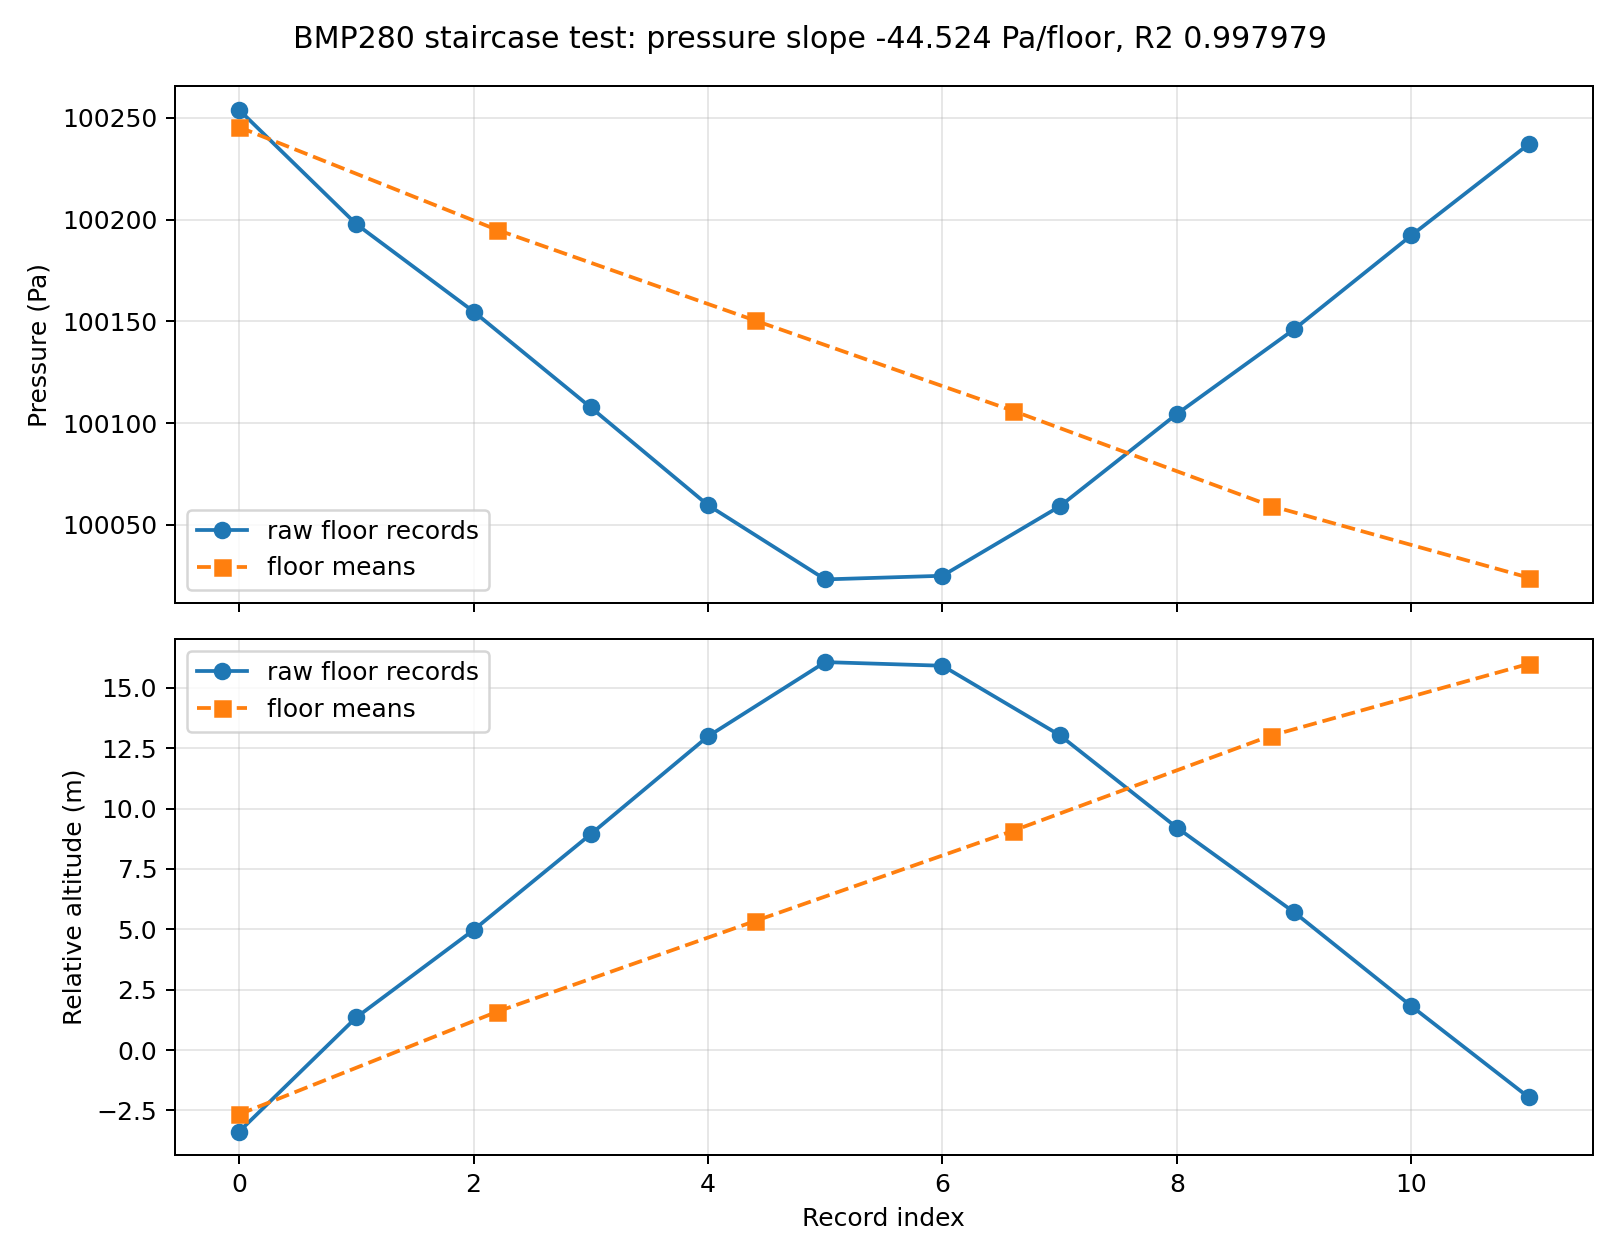
\includegraphics[width=0.95\textwidth]{assets/bmp280_staircase_result.png}
\caption{BMP280 楼梯实验气压--楼层与高度--楼层关系}
\end{figure}

从图中可以看出，气压随楼层升高而近似线性下降，相对高度随楼层升高而近似线性增加。压力拟合 $R^2=0.997979$，高度拟合 $R^2=0.997990$，均满足任务书中 $R^2>0.98$ 的核心验收标准。压力斜率为 -44.524 Pa/层，与理论上每 3 m 约 36 Pa 的量级一致；高度斜率为 3.751 m/层，说明本次测量建筑楼层实际等效高度约为 3.75 m。

\newpage

\section{GPS/气压互补滤波实验}

\subsection{融合算法}

GPS 高度具有绝对参考意义，但其短时噪声和多路径误差较明显；BMP280 气压高度短时连续性较好，但长期会受到天气和参考气压漂移影响。需要注意的是，BMP280 输出的是以开机参考气压 $p_0$ 为零点的相对高度，而 GPS 输出的是海拔高度。二者融合前必须先统一高度基准。本实验以第一条有效 GPS 高度 $h_{\mathrm{gps0}}$ 作为 GPS 基准，先计算 GPS 相对高度：
\begin{equation}
h_{\mathrm{gps,rel}} = h_{\mathrm{gps}} - h_{\mathrm{gps0}}
\end{equation}
然后采用互补滤波将两者结合：
\begin{equation}
h_{\mathrm{fused}} = \alpha h_{\mathrm{baro}} + (1-\alpha) h_{\mathrm{gps,rel}}
\end{equation}
其中，$\alpha=0.98$。该参数表示融合结果主要信任短时平滑的气压高度，同时引入少量 GPS 高度作为绝对参考。

\subsection{实验数据}

GPS/气压融合实验最终有效数据文件为 \texttt{gps\_baro\_0005.csv}。实验在户外开阔环境下静置采集约 15 min，ESP32 同步保存 BMP280 气压高度、GPS 高度、卫星数、HDOP 和融合高度。后处理分析时对 GPS 高度做基准统一，使用 GPS 相对高度参与互补滤波。

\begin{table}[H]
\centering
\caption{GPS/气压互补滤波实验统计结果}
\begin{tabular}{cc}
\toprule
指标 & 结果 \\
\midrule
总采样点 & 4501 \\
采集时长 & 899.751 s \\
GPS 有效样本 & 4499 \\
GPS 有效时长 & 899.654 s \\
平均卫星数 & 5.87 \\
最大卫星数 & 7 \\
平均 HDOP & 1.94 \\
GPS 高度平均值 & 34.829 m \\
GPS 高度标准差 & 8.390 m \\
气压高度标准差 & 0.185 m \\
修正后融合高度标准差 & 0.286 m \\
气压高度变化范围 & 1.337 m \\
\bottomrule
\end{tabular}
\end{table}

\begin{figure}[H]
\centering
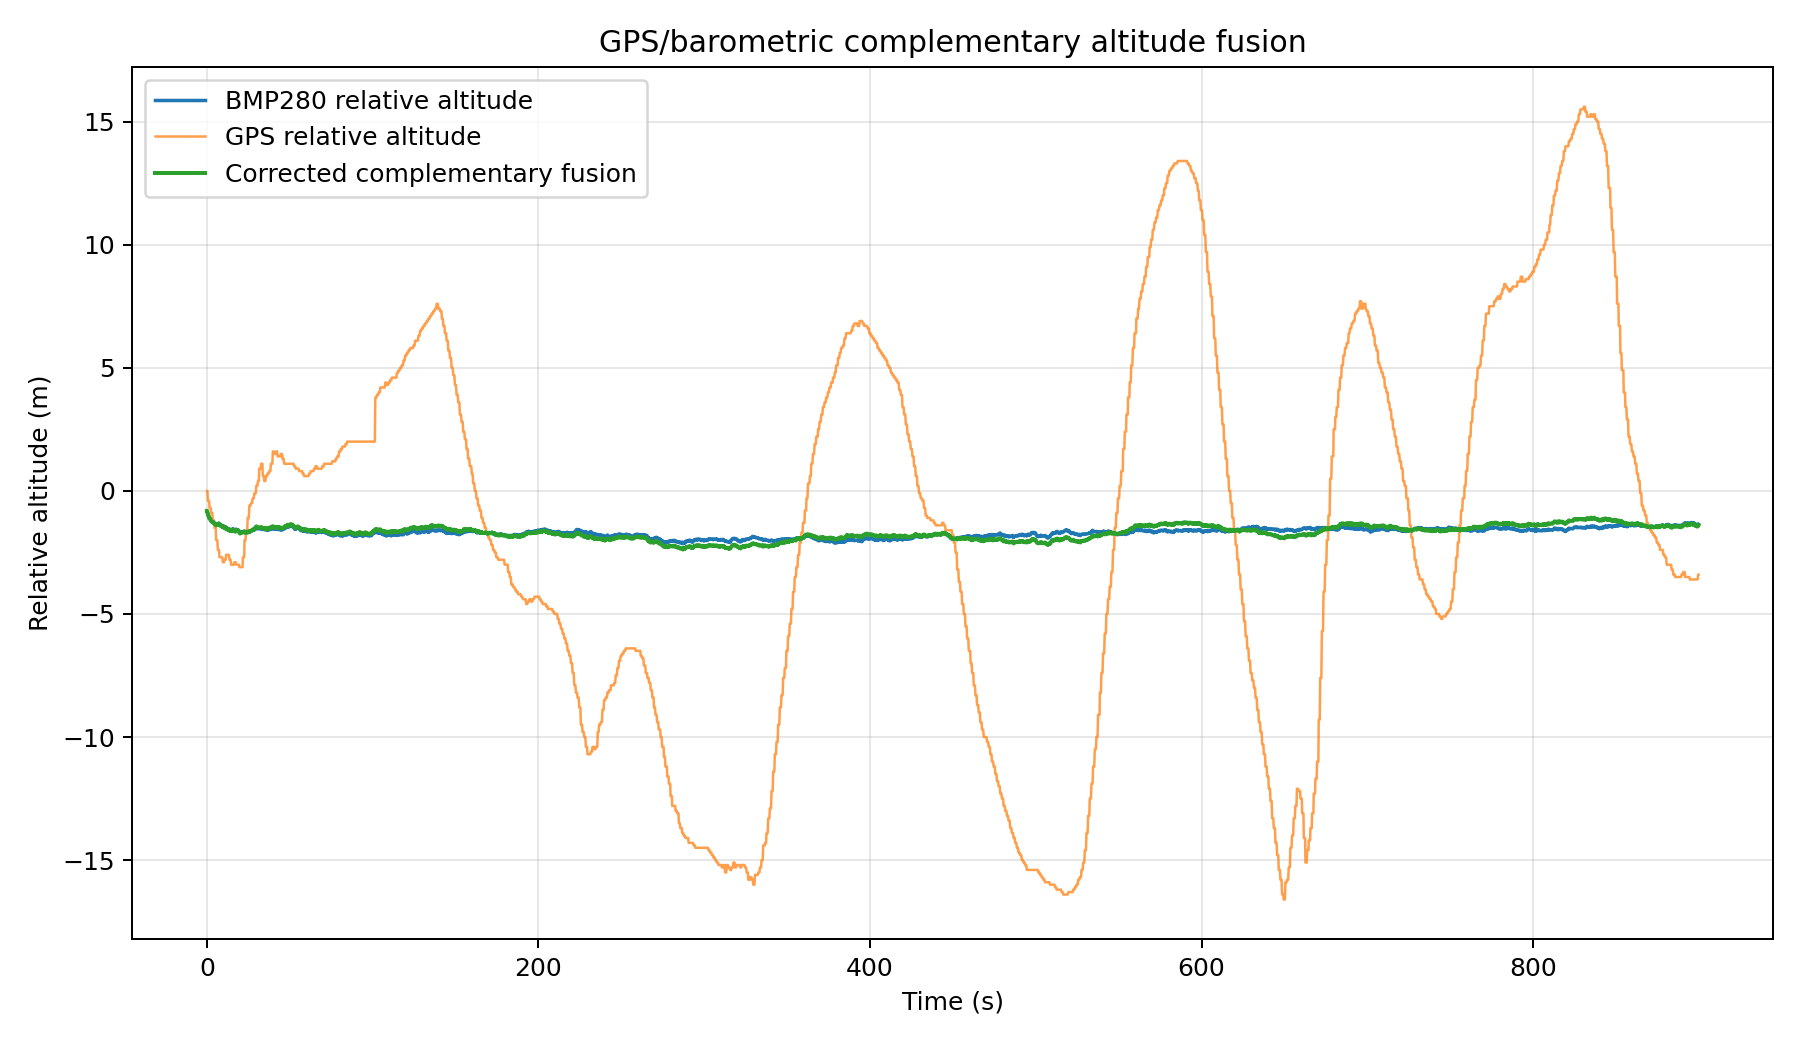
\includegraphics[width=0.95\textwidth]{assets/gps_baro_fusion_height_corrected.png}
\caption{GPS 相对高度、BMP280 气压高度与互补滤波高度对比}
\end{figure}

实验结果显示，GPS 有效时长接近整个采集时长，平均卫星数为 5.87，最大卫星数为 7，平均 HDOP 为 1.94，说明本次户外采集环境满足 GPS 高度分析要求。GPS 高度标准差为 8.390 m，明显大于气压高度标准差 0.185 m，说明静止短时条件下 GPS 高度存在较大波动。基准统一后的互补滤波高度标准差为 0.286 m，远低于 GPS 高度标准差，说明融合结果保持了气压计短时平滑性，同时引入了 GPS 高度的长期参考信息。

\newpage

\section{质量分析}

\subsection{楼梯实验误差}

楼梯实验的误差主要来自以下几个方面：
\begin{enumerate}
  \item 楼梯间开门、人员走动和空气流动会造成局部压力扰动。
  \item 建筑楼层高度并不一定等于理论值 3 m，因此每层气压变化可能与理论 36 Pa/层存在差异。
  \item BMP280 模块靠近 ESP32 和其他器件，温度升高可能影响补偿效果。
  \item 按键后若板子没有完全静止，会引入瞬时压力波动。
  \item 上行和下行之间存在时间间隔，天气系统或室内气压可能发生缓慢漂移。
\end{enumerate}

本实验通过每层采集 30 s 并取平均值、同一楼层上行和下行各测一次并取均值的方式降低随机误差。最终 $R^2$ 接近 0.998，说明数据整体线性较好。

\subsection{GPS/气压融合误差}

GPS 高度误差主要受卫星几何分布、多路径效应、天线姿态和接收环境影响。即使在静止状态下，GPS 高度仍可能出现数米级波动。气压高度误差主要受参考气压 $p_0$、天气变化、温度补偿和气流扰动影响。两者误差特性不同：GPS 更适合提供长期绝对参考，BMP280 更适合提供短时连续高度变化。互补滤波正是利用这两种传感器的互补特性，以较大的权重保留气压高度平滑性，以较小权重引入 GPS 高度参考。

\section{思考题作答}

\subsection{BMP280 补偿算法为什么需要先算温度再算压力？}

BMP280 的压力敏感元件受温度影响明显。Bosch 官方补偿算法在温度补偿阶段计算中间变量 $t\_fine$，该变量不仅用于输出温度，也被压力补偿公式继续使用。如果没有先计算 $t\_fine$，压力补偿算法无法进行温度修正，压力结果会产生系统偏差。因此补偿流程必须是先温度、后压力。

\subsection{楼梯实验中，上行和下行数据一致吗？不一致的原因是什么？}

上行和下行数据总体趋势一致，但同一楼层的气压不会完全相同。不一致原因包括环境气压随时间缓慢漂移、楼梯间开门或空气流动造成瞬时压力扰动、传感器温度逐渐变化、人体移动导致局部气流变化等。本实验对同一楼层的上行和下行数据取平均值，可以减小这类时间漂移和随机扰动的影响。

\subsection{如果在飞机上用 BMP280 测高度，座舱加压后读数会怎样？}

BMP280 测量的是传感器所在位置的局部静压，而不是飞机真实飞行高度。飞机座舱加压后，舱内气压被人为维持在较高水平，因此 BMP280 会根据舱内压力计算出较低的等效高度，不能反映飞机实际高度。在加压舱环境中，气压计测高必须结合舱压系统或外部静压源，不能直接使用标准大气公式。

\subsection{互补滤波的 $\alpha=0.98$ 对应多长时间常数？天气变化快时需要改 $\alpha$ 吗？}

离散互补滤波可近似写为：
\begin{equation}
\alpha = \frac{\tau}{\tau + \Delta t}
\end{equation}
因此：
\begin{equation}
\tau = \frac{\alpha \Delta t}{1-\alpha}
\end{equation}
本实验气压采样频率为 5 Hz，$\Delta t \approx 0.2$ s，当 $\alpha=0.98$ 时，时间常数约为：
\[
\tau = \frac{0.98 \times 0.2}{1-0.98} \approx 9.8\ \mathrm{s}
\]
如果天气快速变化、台风等情况下气压基准漂移较快，应适当降低 $\alpha$ 或周期性用 GPS 高度重新校准 $p_0$，使融合结果能更快修正长期漂移。

\newpage

\section{实验总结}

本实验完成了 BMP280 气压传感器从硬件通信、工厂参数读取、Bosch 补偿算法移植到高度解算和融合应用的完整流程。实验中读取 BMP280 chip\_id 为 0x58，工厂校准参数完整有效。楼梯实验使用 1--6 楼上行和下行共 12 个静止采样点进行验证，压力拟合 $R^2=0.997979$，高度拟合 $R^2=0.997990$，满足任务书要求。GPS/气压融合实验表明，在静止户外环境下 GPS 高度波动明显大于 BMP280 气压高度，互补滤波可以在保留气压高度短时平滑性的同时引入 GPS 绝对高度参考。

总体来看，BMP280 适合用于短时相对高度变化检测，例如楼层变化、台阶爬升和小范围高度变化；GPS 高度适合提供长期绝对参考，但短时噪声较大。二者结合后可以构成低成本的高度估计方案，为后续多传感器融合扩展板中的高度通道提供实验依据。

\section*{附录 A：主要数据文件}
\addcontentsline{toc}{section}{附录 A：主要数据文件}

\begin{longtable}{p{7.0cm}p{7.0cm}}
\caption{实验六主要数据与图表文件} \\
\toprule
文件 & 说明 \\
\midrule
\endfirsthead
\toprule
文件 & 说明 \\
\midrule
\endhead
\path{data/bmp280_staircase/staircase_esp32_0003.csv} & 楼梯实验最终原始数据 \\
\path{data/analysis/bmp280_staircase_summary.csv} & 楼梯实验拟合指标汇总 \\
\path{data/analysis/bmp280_staircase_floor_means.csv} & 6 层楼梯均值表 \\
\path{assets/bmp280_staircase_result.png} & 楼梯实验气压/高度关系图 \\
\path{data/gps_baro/gps_baro_0005.csv} & GPS/气压融合最终原始数据 \\
\path{data/analysis/gps_baro_fusion_summary.csv} & GPS/气压融合统计结果 \\
\path{assets/gps_baro_fusion_height_corrected.png} & GPS 高度、气压高度和融合高度对比图 \\
\bottomrule
\end{longtable}

\end{document}
